\chapter{Wrapping up}

Congratulations! You've reached the end of the journey. But as T. S. Eliot\ia{Eliot, T. S.} reminds us,

\begin{quote}
    In my beginning is my end.\\
    ...\\
    In my end is my beginning.\\
    \citep[177, 183]{Eliot}
\end{quote}

\noindent Indeed, here we are, at the end of this book, but the journey has only just begun. Before you go on to your further adventures, though, it's important to make sure that you have sufficiently processed your experiences from all the recent travels. In this final chapter, we first remind you of the reasons why studying the history of English can be useful and exciting, we then present you with an overview of the main themes we covered, and finally -- as always -- exercises await which should help you to consolidate all that knowledge you picked up along the way.

\section{Main observations}\label{reasons}
We hit the road in \chapref{introduction}, where we discussed six main observations that our voyage was to make us aware of. The remaining chapters then took us to different temporal destinations, in which specific examples relevant for the specific periods were covered.

\subsection{Variation, variation everywhere}
First of all, we saw that variation is indeed omnipresent. All natural languages vary, and variation is found in all areas of the English language. We saw this plenty of times, but let's have a look at some examples. We find examples of orthographic (or spelling) variation:\is{orthography}
\begin{itemize}
    \item Present Day English <you> vs. <u> for \textit{you}
    \item Middle English <whanne> vs. <quanne> for \textit{when} (\sectref{ME-graphical} and \sectref{ME-hdrop})
\end{itemize}

\noindent Phonetic and phonological variation:
\begin{itemize}
    \item Present Day English rising intonation in statements (\ref{HRT})\is{High Rising Terminals}
    \item Old English \textit{hlaf} /hlaːf/ becoming Middle English /laːf/ (\sectref{ME-hdrop})\is{/h/-dropping}
\end{itemize}

\noindent Morphological variation:
\begin{itemize}
    \item Present Day English \textit{The government want to support bumblebee\is{bumblebees} sprees} vs. \textit{The government wants to support bumblebee sprees} {(\sectref{Vconc})}
    \item Middle English pronouns\is{pronouns} \emph{they}, \emph{them} replacing earlier \emph{hie}, \emph{hem} {(\sectref{ME-pronouns})}
\end{itemize}

\noindent Syntactic variation:
\begin{itemize}
    \item Present Day English \textit{My hedgehog got stolen} vs. \textit{My hedgehog was stolen}\is{passive} (\sectref{get-passive})
    \item Early Modern English \textit{What do you read?} vs. earlier \textit{What read you?} (\sectref{EModE-do})\is{\emph{DO}-support}
\end{itemize}

\noindent Lexical variation:
\begin{itemize}
    \item Present Day English \textit{trousers} vs. \textit{pants} (\sectref{lexicon})
    \item \textit{caf\'{e}} referring to a place serving different things in different communities of English (\sectref{lexicon})
    \item Old and Middle English \textit{meat} referring to what today's \textit{food} refers to
\end{itemize}

\noindent And pragmatic variation:\is{historical pragmatics}
\begin{itemize}
    \item Present Day English dialectal terms of address like \emph{love} and \emph{pet} (\sectref{pragmatics})
    \item Middle and Early Modern English second person pronoun\is{pronouns} variation between \emph{thou}/\emph{thee} and \emph{ye}/\emph{you} (\sectref{EModE-pronouns})
\end{itemize} 

\noindent As these examples also demonstrate, we find variation in \textit{all} linguistic levels in all stages of the history of English: Old English, Middle English, Early Modern English, Late Modern English, and Present Day English. And even in the prehistory of the language (\chapref{prehistory}), we can be sure that there was variation, even if not all of it is recoverable by means of linguistic reconstruction.\is{reconstruction}

In addition, we saw that there's another dimension to variation which seeps through language -- the social aspects of language variation. You will, for instance, remember the example of progressive\is{progressive} passives\is{passive} (e.g. \textit{The bumblebees\is{bumblebees} are being watched}) being (a) heavily stigmatized in Late Modern English; and (b) associated with the group of the Lake Poets.\is{poetry} As speakers of Present Day English, we know that progressive\is{progressive} passives\is{passive} are (a) no longer stigmatized, and (b) no longer associated with the Lake Poets. Linguistic variation can serve a wide range of functions, and the social meaning of variation is also subject to change.

\subsection{The social life of language}
In every period of the language, it therefore also became apparent that linguistic variation more often than not comes with a certain social function, or social meaning. In other words, although many instances of linguistic variation do not change the lexical content of a sentence, they can reveal various social affiliations of the speakers. We discussed this most in the chapter on Present Day English, where it's easiest to tap into such social meanings of linguistic variation, but there's no doubt that cases of variation in the older periods also went hand in hand with variably complex social implications.

To refresh our memory a little bit here, remember the stigma associated with \glossterm{gl-hdrop}{/h/-dropping}\is{/h/-dropping} discussed in \chapref{LModE}, related to one's social class and therefore status in the power dynamics of the social hierarchy. We also touched upon the case of AAE (African American English),\il{English, African American} whose linguistic features typically signal one's ethnicity. But even something as innocuous as spelling\is{orthography} can signal social meaning; can you imagine your grandparents writing \textit{C u l8er!} to you, or some such? To combine a range of linguistic phenomena clearly imbued with social meaning, imagine your grandparents writing \textit{S'up, bro?} when communicating with you.

\subsection{Irregularities}\is{irregularities|(}
Within standard (and most non-standard) varieties of English, in Chapters \ref{EModE}--\ref{prehistory} we read about changes and alternations that have resulted in the following irregularities:

\begin{itemize}
    \item irregular plural\is{plurals} formation: \textit{child} $\sim$ \textit{children}; \textit{man} $\sim$ \textit{men}; \textit{ox} $\sim$ \textit{oxen}; \textit{sheep} $\sim$ \textit{sheep}; \textit{wolf} $\sim$ \textit{wolves} 
    \item irregular verbal inflection:\is{inflection} \textit{drink} $\sim$ \textit{drank} $\sim$ \textit{drunk}; \textit{keep} $\sim$ \textit{kept} $\sim$ \textit{kept}
    \item irregular comparatives and superlatives: \textit{old} $\sim$ \textit{elder} $\sim$ \textit{eldest}\footnote{These coexist in most varieties of English with the regular (and more frequently\is{frequency} used) forms \emph{older} and \emph{oldest}.}
    \item not numerous but frequent noun-adjective correspondences: \textit{length} $\sim$ \textit{long}; \textit{sanity} $\sim$ \textit{sane}
    \item not numerous but frequent noun-verb correspondences: \textit{song} $\sim$ \textit{sing}; \textit{tooth} $\sim$ \textit{teethe}
\end{itemize}

\noindent Many more examples were provided in the relevant chapters, and now you're less in the dark as to where they come from. And if you're still as much in the dark as before starting reading this book, we recommend revisiting the chapters, especially if it's been some time between your last classes and your exam preparation. And remember there's always the table of contents to consult in order to remind yourself where we discuss what.\is{irregularities|)}

\subsection{Interpreting older literary and other texts}
In \chapref{EModE}, it started becoming apparent that we need to know at least something about the language of the period to be able to engage with the literary (and other) works of Early Modern English. More specifically, we saw that the 2nd person pronoun\is{pronouns} variation went with a complex web of social meanings (remember our \textit{you}, \textit{thou}, and \textit{thee} examples and the Hamlet exercise, \ref{ex-thou}), which are likely lost on the reader of the 21st century without sufficient knowledge of the history of English.

Further down the path, the language started to look somewhat alien as we approached Middle English and even more so by the time we reached Old English. Without a dictionary\is{dictionaries} and a basic knowledge of the structural properties of the language, we would all find it extremely challenging, if not impossible, to even read texts written in Middle and Old English, let alone engage with them further beyond basic comprehension.

\subsection{Different linguistic levels can interact}
We also saw that the different linguistic levels or domains (morphology, syntax, phonology, lexicon, pragmatics) not infrequently interact with each other. To take a Present Day English example, in Exercise \ref{exercise-variation} in \chapref{introduction} we saw a sentence containing \textit{I dunno}. As the non-standard spelling\is{orthography} implies, this is not pronounced as [aɪ dəʊnt nəʊ] (which is what the standard spelling, <I don't know>, would suggest), but rather something like [ɐdənə]. So here we see something very much related to sounds and phonology. However, all these reductions\is{vowel reduction} also affect the morphology of the phrase: how many words are there in something like \textit{I dunno}? If we decided to treat \textit{dunno} as a single word, this also means that there is a new lexical item in one's vocabulary, and so we would have to also consider this of relevance for the lexical component of English. This makes this example also relevant for syntax: depending on how many words we say \textit{dunno} represents, and the structure that underlies it, we'd have to conceptualize these different possibilities with different syntactic analyses and trees.\is{syntactic trees} And finally, pragmatics\is{historical pragmatics} also gets to share in the interest surrounding \textit{I dunno}. For instance, \citet{PichlerLevey2010} show that the reduced form, \textit{dunno}, is associated with different pragmatic functions than the unreduced form, \textit{I don't know}: in their data, in doctor-patient conversations the reduced form was associated with reluctance to talk as opposed to genuine lack of knowledge.

In the previous chapters, you were presented with more examples which would be of interest to a range of linguists interested in various levels, such as semi-modals\is{modals} discussed in \chapref{LModE} on Late Modern English (\textit{gonna}, \textit{finna},\is{\emph{fixing to} (\emph{finna})} etc.), the Great Vowel Shift\is{vowels}\is{Great Vowel Shift} discussed in \chapref{EModE} on Early Modern English, and the reduction of morphological endings discussed in Chapters \ref{ME} and \ref{OE} on Middle and Old English. And those are just some of the many examples we could recall here.

If, at this stage, you are worried about not being able to tell whether a certain phenomenon belongs to the domain of syntax or morphology or phonology, etc., we recommend calming down with a cup of good tea (or cake, or both), consulting the list of contents of this book (which gives you a list of phenomena under the linguistic domains), and realizing that more often than not a specific case of language change is of relevance to multiple domains of language structure. Interaction between various linguistic levels happens all the time, and there is no hiding from this fact.

\subsection{Language change is inevitable (and perfectly normal)}
And by this point, you might be thinking that we've been hammering this message home a wee bit too much, but here it comes again, because it \textit{is} important: language change is inevitable -- and perfectly normal. We saw this in every stage of the history of the English language. This fact enables us to make interesting observations.

First, what we learn about the mechanisms of language change in Present Day English should also hold for how change can operate in earlier stages of the language. This also works the other way round. In other words, if we think that a certain change is impossible or unlikely in Present Day English, it should also be impossible or unlikely in all previous stages, and vice versa. To use T. S. Eliot's\ia{Eliot, T. S.} insights again,

\begin{quote}
    Time present and time past\\
    Are both perhaps present in time future\\
    And time future\is{futurity} contained in time past.\\
    \citep[171]{Eliot}
\end{quote}

\noindent It is sometimes the case that efforts at standardization\is{standardization} and codification, of the kind discussed in \chapref{EModE}, may explicitly aim to halt -- or even reverse -- language change. However, they are basically never successful in doing so -- although deliberate efforts at prescriptivism\is{prescriptivism} may have other, unintended effects \citep{Curzan2014}.

The second observation we can make is that it seems very usual for human beings to comment on language, and to be anxious and self-conscious about our own language use. We mainly looked at this in \chapref{LModE} and to some extent in \chapref{englishtoday}. If you're interested in a critical approach to these topics, we recommend \citet{Cameron2003}, and for a perspective from the history of English see \citet{Machan2009}.\\

\noindent So here we are, having reminded ourselves of the major observations about how one could benefit from studying the history of a language, and in our case that of English. And who knows, perhaps you can think of even more reasons!

\section{Themes}

We've seen that there are good reasons why one would want to study the history of English. As we navigated through the different periods (moving from the comforts of Present Day English to the rougher seas of Germanic), we also encountered several themes which are important for our understanding of how the language has developed. \sectref{reasons} touched upon some of these, but let's remind ourselves of all of the major themes now.

As already mentioned, variation is omnipresent. It appears on all linguistic levels and in all historical periods of the language (and languages other than English are no exception, of course barring languages that are dead). This leads us to the first theme: homogeneity vs. heterogeneity. In \chapref{englishtoday}, we mentioned how dialects of English are often seen as dying out due to the effects of media\is{media} and technology.\is{technology} We saw plenty of examples of changes which happen in a (more) global\is{globalization} scale in English as well; however, these typically (if not always) develop local ``flavours''. While older varieties of English may be changing, that does not necessarily mean they are dying out. And even in cases where some traditional dialects could be considered extinct or significantly changed in terms of their perceived salience, new dialects do develop. Homogeneity and heterogeneity are therefore relative. And if we remember \chapref{LModE}, where the emergence of American English\il{English, American} was introduced, we find a very good example thereof.

In a similar vein, while the technological\is{technology} developments we've experienced across the past decades and centuries have changed how we communicate, the research available thus far suggests that exposure to TV and social media\is{media} do not lead to language change as much as is frequently assumed by the general public (see \chapref{englishtoday}).

Chapters \ref{introduction} and \ref{englishtoday} also introduced the sentiment expressed by a wide range of speakers: language change is seen as bad. This theme also appeared in \chapref{LModE}. Indeed, the idea that change is bad is a fairly widespread belief, and one which is by no means limited to language.\footnote{George and M\'{i}\v{s}a, for instance, both refused to buy a smartphone for a long time (although they would grudgingly admit the advantages of owning one of the machines). George finally surrendered to the smartphone technology\is{technology} in summer 2021, while  M\'{i}\v{s}a is still holding on.} However, throughout the book we were again and again exposed to different waves of changes, and one thing that does remain constant as we travel through the historical stages of English is the fact that all the linguistic levels will and do undergo changes of some sort. Change is inevitable, whatever we may think of it as speakers.

This leads us to a very closely related topic, that of prescriptivism.\is{prescriptivism} Prescriptivism was the overarching theme of \chapref{LModE}. Although the phenomenon is not limited to Late Modern English, it is very much felt in this period in particular, in contrast to the older periods. In \chapref{EModE}, we were predominantly occupied with the theme of standardization,\is{standardization} which turned out to be very important for the rise of institutionalized prescriptivism in the history of English, and in Late Modern English in particular.\is{prescriptivism}

\chapref{ME} was very much about transitions.\is{transition problem} The Middle English period, before standardization\is{standardization} got into full swing, is hugely diverse in terms of the linguistic varieties attested, and drastic changes can be observed on all linguistic levels in the four hundred years of Middle English. /h/s\is{/h/-dropping} were lost left, right and centre,\is{consonants} a smorgasbord of new pronouns\is{pronouns} made their way into the language from different sources, and verb-second\is{verb-second} word order gave way to the subject-verb-object (SVO)\is{subjects} word order\is{word order} of the present-day language. Some of these transitions are predictable as part of larger patterns: for instance, the meaning change of \emph{indeed}, where originally pragmatic meaning becomes semantically encoded,\is{historical pragmatics} a common tendency in language change. Others, like vowel lengthening\is{vowel lengthening} and shortening\is{vowel shortening} processes,\is{vowels} can seem arbitrary and idiosyncratic. The history of any language is filled with both kinds of transition.\is{transition problem}

In \chapref{OE}, we focused on language contact and multilingualism.\is{multilingualism} When approaching Old English, and the change from Old English to Middle English, it is important for us to consider the role of contact with Brythonic Celtic,\il{Celtic, Brythonic} \ili{Norse}, and \ili{Latin} (at least). Although we emphasized language contact in our discussion of Old English, we also saw that language contact played an important role in Middle English (\ili{Latin} and \ili{French} being the most frequently highlighted languages of interest). Starting with colonization\is{colonialism} in Early Modern English, language contact with a wide range of cultures and speakers of different languages has introduced a good range of new concepts, words and structures into the language. The English language has never stood ``alone'', and it has never been the province of only monolinguals, despite what nationalistic ``one nation,\is{nation-states} one language'' rhetoric would have us believe.

Finally, \chapref{prehistory} dealt with linguistic prehistory. The issues raised there about our access to knowledge are crucial for any reflection on history: how do we find out about the past? And how can we find out whether we're right? Regardless of whether we have preserved texts from a particular period or not, do we ever really have direct access to the truth of what happened? Our stance -- the stance of all serious historians -- is that the story we tell is constructed. The title of the book is ``\emph{A} history of English'', with an indefinite article,\is{articles} not ``\emph{The} history of English'', with a definite article. Our history, like all other possible histories, is a narrative, one that we've put together in good faith and with the aim of coming as close to the truth as possible. But, like all other possible histories, our history is subjective, coloured by who we are as writers, and what you take away from your journey will also be subjective, coloured by who you are as a reader. There exist mountains of scholarship in English historical linguistics, and we have had to be selective in what we include. It's also important to remember that the history of English is not a closed book: new evidence is still coming to light, and new interpretations of old evidence are frequently proposed. Just like the English language itself, the received wisdom as to the history of the language is variable, and constantly in flux.

Having reached the final destination and packed with knowledge, you're presented with a little snack to help you consolidate all this knowledge (and possibly get ready for your exam, if you're taking a course on the history of English).

\addsec{Suggested exercises}
\begin{exercises}{Variation everywhere?}
List two examples of variation found in Present Day English regarding:
\begin{enumerate}
      \item orthography/spelling\is{orthography}
      \item phonetics and phonology
      \item morphology
      \item syntax
      \item lexicon
      \item pragmatics/discourse
\end{enumerate}

\noindent Don't be surprised if some of your examples seem to bridge more than one linguistic level (e.g. both morphology and syntax, or both morphology and phonology).

\end{exercises}


\begin{exercises}{The Sower and the Seed revisited}\label{sower-and-seed-2}
Below are four versions of the Parable of the Sower and the Seed from the New Testament (Matthew 13, verses 3--4), from different points in time, across a thousand years of the history of English. This exercise is repeated from \chapref{introduction} (\sectref{sower-and-seed}). If you did it then, it's worth revisiting now in order to reflect on how much you've learned. If you didn't do it then, well, it's still a good exercise!

\begin{itemize}
    \item \textit{A farmer went out to sow his seed. As he was scattering the seed, some fell along the path, and the birds\is{birds} came and ate it up.}\\ 
	(New International Version, 1973)
    \item \textit{Behold, a sower went forth to sow; And when he sowed, some seeds fell by the way side, and the fowls came and devoured them up.}\\ 
	(King James\ia{Stuart, James (King James I)} version, 1611)
    \item \textit{Lo! he that sowith, yede out to sowe his seed. And while he sowith, summe seedis felden bisidis the weie, and briddis of the eir camen, and eeten hem.}\\
	(Wycliffe\ia{Wycliffe, John} version, c. 1395)
    \item \textit{Soþlice ut eode se sædere hys sæd to sawenne and þa þa he seow. sume hig feollon wiþ weg. and fuglas comun and æton þa;}\\
    (West Saxon\il{Old English, West Saxon} Gospels, c. 990)
\end{itemize}

\noindent Try to identify differences between the texts in terms of each of the linguistic levels we've discussed in the book:
\begin{itemize}
    \item Phonetics \& phonology\\ 
    (of course, here you'll need to make an educated guess, based on spelling)\is{orthography}
    \item Morphology
    \item Syntax
    \item Lexicon
    \item Pragmatics/discourse
\end{itemize}

\noindent \emph{Tips for teachers:} If you'd like to make this exercise a bit more novel, replace these specific extracts with other ones, or add some more.

\end{exercises}

\largerpage
\begin{exercises}{Timeline}
Below is a blank timeline covering the years 400 to the present. Print it out or photocopy it, and try to fill in the timeline with important events and changes in the history of English. If you find it useful, you can distinguish between historical changes that are relevant for the history of the language (like the Norman Conquest)\is{Norman Conquest} and changes in the language itself (like the Great Vowel Shift)\is{vowels}\is{Great Vowel Shift} by putting historical events above the line and language changes below the line.\newpage

\begin{figure}[H]
\vspace*{2cm}
          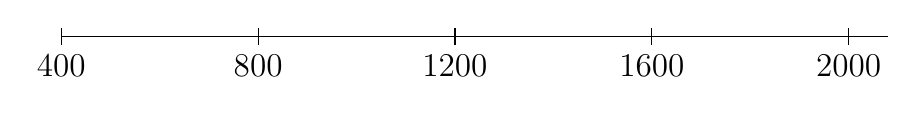
\begin{tikzpicture}
      \draw (0,0) -- (10.5,0);
      \foreach \x in {0, 2.5, 5, 7.5, 10}
      \draw (\x cm,3pt) -- (\x cm,-3pt);
      \draw (0,0) node[below=3pt] {\large{400}};
      \draw (2.5,0) node[below=3pt] {\large{800}};
      \draw (5,0) node[below=3pt] {\large{1200}};
      \draw (7.5,0) node[below=3pt] {\large{1600}};
      \draw (10,0) node[below=3pt] {\large{2000}};
     \end{tikzpicture}
\vspace*{2cm}
\end{figure}

\noindent\emph{Tip for students}: This works well as a revision exercise.\\

\noindent\emph{Tip for teachers}: In class, this exercise can be carried out in small groups. Give the students 20--30 minutes to put the timeline together, then compare the results in plenary.\\

\noindent\emph{Tip for teachers}: Different groups will have different timelines, and not all of the differences will be straightforwardly errors. You can use this to start a discussion about the subjective nature of history-telling, if appropriate.\\

\noindent\emph{Tip for teachers}: If students have included historical figures (Shakespeare,\ia{Shakespeare, William} Alfred,\ia{Alfred (King of Wessex)} Columbus...)\ia{Columbus, Christopher} on their timelines, you can also use this to start a discussion about gender representation in history-telling and the reasons behind this.\is{gender studies}

\end{exercises}

\begin{exercises}{Irregularities}
Think of three to five irregularities\is{irregularities} in Present Day English. Can you say anything about where these irregularities come from?
\end{exercises}

\begin{exercises}{Food for thought}
``Consider one aspect of the history of English for which we don't have completely sufficient evidence and, on the basis of this example, discuss the challenges of trying to learn about a language from the past. How have scholars tried to meet these challenges regarding this aspect of the history of English, and how successful have been their attempts?'' \citep[104]{Liu2019}

\end{exercises}

\begin{flushright} {\color{magenta}\textit{Fare well, and may the bumblebees be with you!}}\is{bumblebees}\\

\noindent {\color{magenta}\textit{Míša and George}}
\end{flushright}
